\documentclass{article}
\usepackage[utf8]{inputenc}
\usepackage{graphicx}
\usepackage{fancyhdr}
\usepackage{geometry}
\usepackage{amsmath}
\usepackage{amssymb}


\geometry{left = 2.5cm, right=2.5cm, bottom=2.5cm, top=2.5cm}

\title{3806ICT - Week 2 Lab}
\author{Nick van der Merwe - s5151332 - nick.vandermerwe@griffithuni.edu.au}

\pagestyle{fancy}
\renewcommand{\headrulewidth}{1pt}
\fancyhf{}
\rhead{2802ICT - Assignment 2}
\chead{Griffith University}
\lhead{Nick van der Merwe - s5151332}
\rfoot{Page \thepage}

\begin{document}
\maketitle

%==============================================================================
\section{Task 1 - Explain ROS}
\subsection{What is a ros node?}

A ros node is an executable in a ros package which communicates through topics to one another.

%==============================================================================
\subsection{What is roscore?}

Roscore essentially hosts all the nodes that are running on ros. For any nodes to communicate, ros must be running. 

% 3==============================================================================
\subsection{What is the difference between publisher/subscriber and a service?}

A publisher sends information to a topic, a subscriber reads information from a topic and 
a service is a node that can be requested to reply with information.

% 4
\subsection{What is the purpose of catkin?}
Catkin is a build system that manages workspaces, and within those, packages, and compiling them.

% 5
\subsection{What does the roscd command do?}
Like the cd command in linux, it navigates to the given package or stack in the ros system.

% 6
\subsection{Show the command for creating a package called lab2 which relies on roscpp, rospy, std\_msgs and message\_generation}
I've already ran it, but its catkin\_create\_pkg lab2 roscpp rospy std\_msgs message\_generation
% 7
\subsection{What do I have to change in my package.xml file to enable message generation?}
Its required to uncomment the \textless build\_depend \textgreater message\_generation\textless/build\_depend\textgreater line and the \textless exec\_depend \textgreater message\_runtime\textless /exec\_depend\textgreater (excuse the weird latex spaces).
% 8
\subsection{What is the difference between a msg and a srv file?}
A msg file, or message file, is used to define the format of the messages being communicated whereas services 
describe the format of a service. A srv is split into two sections, a request and a reponse.

% 9
\subsection{Define what these types represent}
\subsubsection{uint32}
An unsigned int made of 32 bits or 8 bytes - the same as uint32\_t
\subsubsection{string}
An array of characters, a std::string
\subsubsection{float64}
A float made of 64 bits - a double.
\subsubsection{float32}
A float made of 32 bits - a float.
\subsubsection{bool}
A boolean value - uint8\_t - Quick question, wouldn't it have been better if ros actually used a bool type since std::vectors 
are optimised to compress them? Do some robots really have a 1 bit bool or something?
\subsubsection{int64}
An int made of 64 bits - int64\_t
\subsubsection{int32}
An int made of 32 bits - int32\_t

\section{Task 2 - Programming Exercise}
This is explained... oddly. Here's my list of assumptions
\begin{itemize}
    \item The origin is always the same (5.54445). After reading the turtle sim source code, This
    seems to always be the case as its based on the resolution of the turtle and we can assume that's constant.
    \item Zero degrees occurs at the far right - like a unit circle system. The way that quadrants are usually defined
    \item The edge case of when the turtle is exactly on a border between two
    is that it belongs to the one more upper right. For instance if its between 
    quadrant 1 and 2 then it belongs to 1.
\end{itemize}

So here's the result.
\newpage

\begin{figure}[h]
    \caption{The publisher}
    \centering
    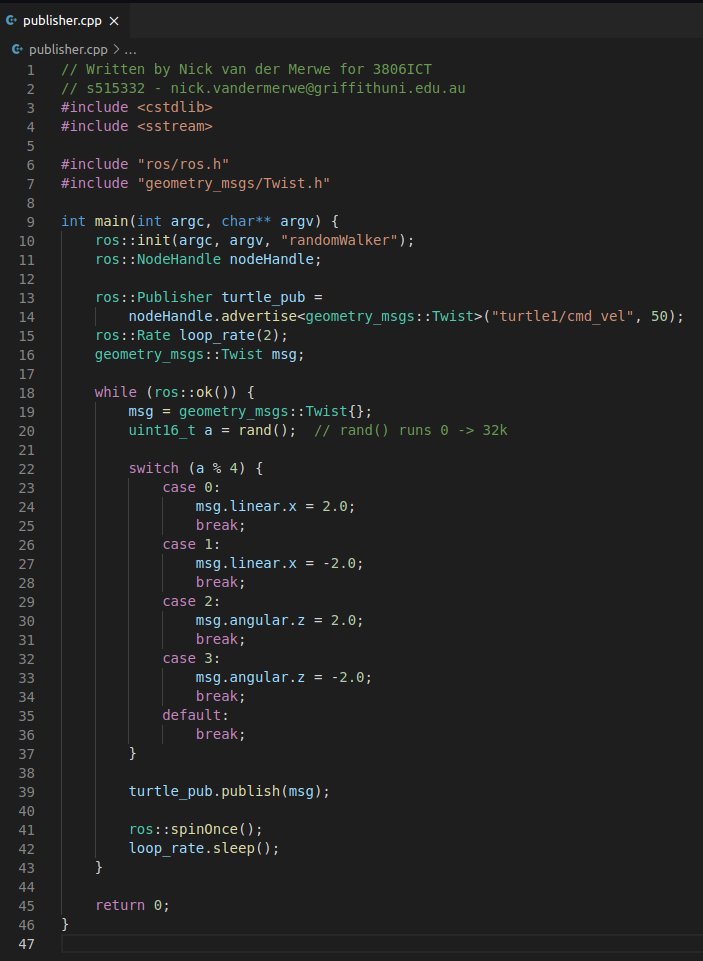
\includegraphics[width=1\textwidth]{img/publisher.png}
\end{figure}

\begin{figure}[h]
    \caption{The subscriber}
    \centering
    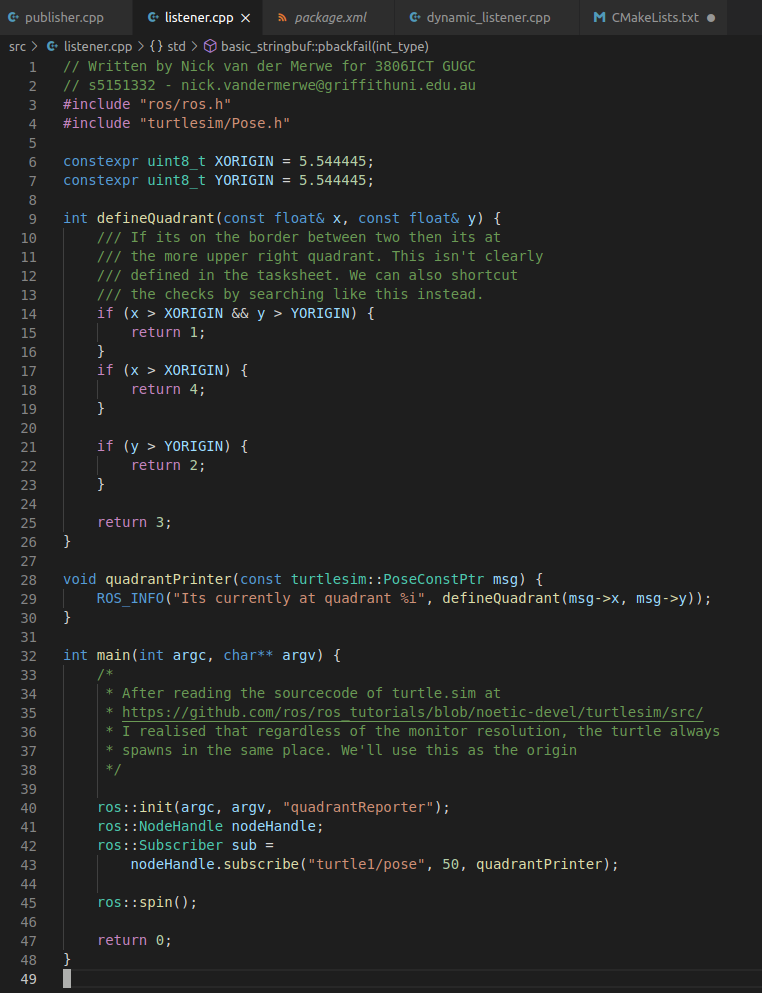
\includegraphics[width=1\textwidth]{img/listener.png}
\end{figure}

\begin{figure}[ht]
    \caption{Everything in action}
    \centering
    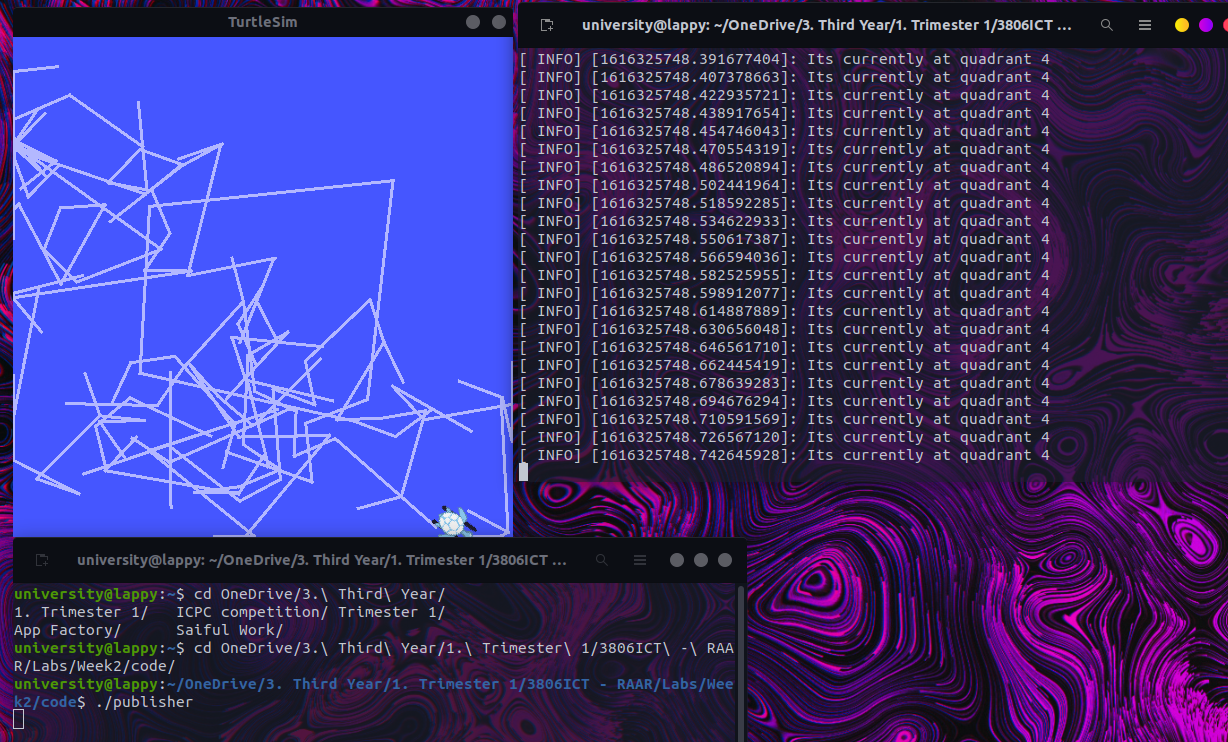
\includegraphics[width=1\textwidth]{img/inAction.png}
\end{figure}

In retrospect, I probably should've just merged both the publisher and subscriber into the same file. With that being said, this is how the ros wiki tutorials made these.

\end{document}
